\documentclass[aspectratio=169]{beamer}

\definecolor{cardinal}{RGB}{140,21,21}
\definecolor{offblack}{RGB}{46,45,41}
\definecolor{cloud}{RGB}{218,215,203}
\definecolor{driftwood}{RGB}{182,177,169}
\usetheme[progressbar=frametitle,sectionpage=progressbar]{metropolis}
%\usetheme[progressbar=frametitle,sectionpage=progressbar]{metropolis}

%\setbeamercolor{palette primary}{bg=cardinal,fg=white}
%\setbeamercolor{palette secondary}{bg=cardinal,fg=white}
%\setbeamercolor{palette tertiary}{bg=cardinal,fg=white}
%\setbeamercolor{palette quaternary}{bg=cardinal,fg=white}
%\setbeamercolor{structure}{fg=cardinal} % itemize, enumerate, etc
%\setbeamercolor{section in toc}{fg=cardinal} % TOC sections

\setbeamercolor{normal text}{bg=white,fg=offblack}
\setbeamercolor{frametitle}{fg=white,bg=cardinal}
\setbeamercolor{progress bar}{fg=white,bg=white}
\setbeamercolor{title separator}{fg=cardinal}
%\setbeamercolor{progress bar in head/foot}{bg=cardinal,fg=white}
\setbeamercolor{progress bar in section page}{fg=cardinal,bg=driftwood}
\setsansfont[BoldFont={Source Sans Pro Semibold}, RawFeature={+kern, +ss01, +lnum, +liga, +tlig},
             SmallCapsFont={Source Sans Pro}, SmallCapsFeatures={Letters=SmallCaps}]{Source Sans Pro}
\setmonofont{Source Code Pro}
\newfontfamily{\halfbf}{Source Sans Pro Semibold}[RawFeature={+kern, +ss01, +liga, +tlig}]
\DeclareTextFontCommand{\texthalfbf}{\halfbf}
\newfontfamily{\fullbf}{Source Sans Pro Bold}[RawFeature={+kern, +ss01, +liga, +tlig}]
\DeclareTextFontCommand{\textfullbf}{\fullbf}
\newfontfamily{\doublebf}{Source Sans Pro Black}[RawFeature={+kern, +ss01, +liga, +tlig}]
\DeclareTextFontCommand{\textdoublebf}{\doublebf}
\usepackage{tabu}
\usepackage{pgfplots}
\usepackage{pgfplotstable}
\usepackage{graphicx}
\usepackage{textpos}
\usepackage{savesym}
\savesymbol{checkmark}
\usepackage{dingbat}
\usepackage{booktabs}
\usepackage{array}
\usepackage{siunitx}
\sisetup{detect-all}
\usepackage{multirow}
\usepackage{tikz}
\usepackage{calc}
\usetikzlibrary{calc}
\usepackage{outlines}

\definecolor{CB-Pl-blue}{HTML}{a6cee3}
\definecolor{CB-Pd-blue}{HTML}{1F78b4}
\definecolor{CB-Pl-green}{HTML}{b2dF8a}
\definecolor{CB-Pd-green}{HTML}{33a02c}
\definecolor{CB-Pl-red}{HTML}{Fb9a99}
\definecolor{CB-Pd-red}{HTML}{e31a1c}
\definecolor{CB-Pl-orange}{HTML}{FdbF6F}
\definecolor{CB-Pd-orange}{HTML}{FF7F00}
\definecolor{CB-Pl-purple}{HTML}{cab2d6}
\definecolor{CB-Pd-purple}{HTML}{6a3d9a}
\definecolor{CB-Pl-brown}{HTML}{FFFF99}
\definecolor{CB-Pd-brown}{HTML}{b15928}
\pgfplotscreateplotcyclelist{PairedLightDark}{%
  {CB-Pd-blue,draw=none},
  {CB-Pl-blue,draw=none},
  {CB-Pd-green,draw=none},
  {CB-Pl-green,draw=none}}
\pgfplotscreateplotcyclelist{PairedLightDarkLines}{%
  {CB-Pd-blue,solid,thick},
  {CB-Pd-green,densely dotted,very thick},
  {CB-Pd-red,densely dashed,thick},
  {CB-Pd-brown,solid,very thick},
  {CB-Pd-purple,densely dotted,thick},
  {CB-Pd-orange,densely dashed,thick}}

% Tikz global options
\tikzset{every picture/.style={/utils/exec={\small\sffamily}}}

% Tikz named styles
\tikzstyle{hairline}=[very thin,draw=gray]
\tikzstyle{line}=[semithick]
\tikzstyle{arrow}=[line,->,>=latex]

\pgfplotsset{compat=1.13}
%\usepackage[duration=15,lastminutes=2]{pdfpcnotes}
\renewcommand{\emph}[1]{\textcolor{cardinal}{{\halfbf #1}}}

\newcommand*{\lhand}[2]{
  \only<.(1)> {
  \begin{textblock}{2}(#1,#2)%
    \LARGE%
    \textcolor{cardinalred} {%
    \rightpointleft%
    }%
  \end{textblock}%
  }
}
\newcommand*{\rhand}[2]{
  \only<.(1)> {
  \begin{textblock}{2}(#1,#2)%
    \LARGE%
    \textcolor{cardinalred} {%
    \leftpointright%
    }%
  \end{textblock}%
  }
}
\newcommand*{\uhand}[2]{
  \only<.(1)> {
  \begin{textblock}{2}(#1,#2)%
    \LARGE%
    \textcolor{cardinalred} 
    }%
  \end{textblock}%
  }
}
\newcommand*{\dhand}[2]{
  \only<.(1)> {
  \begin{textblock}{2}(#1,#2)%
    \LARGE%
    \textcolor{cardinal} 
    }%
  \end{textblock}%
  }
}

\makeatletter
\def\convertto#1#2{\strip@pt\dimexpr #2*65536/\number\dimexpr 1#1}
\makeatother

\pgfplotsset{
    %/pgfplots/area legend/.style={%
    %    /pgfplots/legend image code/.code={%
    %        \fill[##1] (0cm,-0.1cm) rectangle (0.6cm,0.1cm);
    %    }%
    %},
    global/.style={
      set layers,
      font=\footnotesize\sffamily,
      cycle list name=PairedLightDark,
      legend style={
        /tikz/every even column/.append style={column sep=0.5pc},
        draw=none
      },
      %cycle list shift=4,
      %xticklabel={$\mathsf{\pgfmathprintnumber{\tick}}$},
      minor grid style={line width=.2pt, draw=gray!25},
      enlarge x limits=0.2,
%tick label style={/pgf/number format/assume math mode=true}
    },
    globother/.style={
      global,
      yticklabel={$\mathsf{\pgfmathprintnumber{\tick}}$},
    },
    barmixin/.style={
      bar width=6pt,
      area legend,
      log origin=infty,
      ymajorgrids=true,
      yminorgrids=true,
      yminorticks=true,
    },
    logbarstyle/.style={%
      global,
      every axis plot/.append style={fill, on layer=pre main},
      /pgfplots/log number format basis/.code 2 args={$\mathsf{##1^{\pgfmathprintnumber{##2}}}$},
      barmixin,
    },
histstyle/.style={
    width=0.60\paperwidth,
    height=0.75\paperheight,
    ylabel={Count}, 
    xlabel={Issued per Cycle},
    legend style={
      legend columns=1,
      at={(1.10,0.5)},
      anchor=west,
    },
    legend cell align={left},
    global,
    cycle list name=PairedLightDarkLines,
      enlarge x limits=0.0,
    ymin=0,
    ymax=75000,
},
    globbar/.style={
      global,
      every axis plot/.append style={fill, on layer=pre main},
      yticklabel={$\mathsf{\pgfmathprintnumber{\tick}}$},
      ytick style={draw=none},
      barmixin,
    },
    tighty/.style={
ylabel shift = .25pc
} 
}



\title{{\Huge \doublebf Capstan}}% {\Huge \bf [eRSS]}}
\subtitle{{\Large Regular Hardware for Irregular Problems}}
\author{{\halfbf{Alexander Rucker}}\\
Stanford University}
%\date{September 11, 2019}

\titlegraphic{\hfill 
\includegraphics[scale=0.20]{SU_Seal_Red_darkbgrd.eps}}
\newlength{\zeroheight}
\newcommand{\sparkbar}[3]{\textcolor{CB-Pd-blue}{\rule[0.5\zeroheight-1ex*\real{0.5}]{#2*\real{#1}/\real{#3}}{1ex}}}

\newcolumntype{L}[1]{>{\raggedright\arraybackslash}p{#1}}
\newcolumntype{C}[1]{>{\centering\arraybackslash}p{#1}}
\newcolumntype{R}[1]{>{\raggedleft\arraybackslash}p{#1}}

\begin{document}
\maketitle
\if 0
\begin{frame}
  Height: \convertto{in}{\the\paperheight} in

  Width: \convertto{in}{\the\paperwidth} in
\end{frame}
\fi
\begin{frame}
  \frametitle{Goals}
    \begin{outline}
      \1 Reconfigurability
      \2 Built on Plasticine fabric
      \2 Maintain PMU/PCU abstraction
      \pause
      \1 Performance
      \2 High-throughput issue logic
      \2 Outer-parallelization support
      \pause
      \1 Programmability
      \2 Understandable memory model
    \end{outline}
\end{frame}
\begin{frame}
  \frametitle{Bank allocation for high throughput}
  \centering
  \includegraphics[scale=2.0]{sparse_read_pipe.png}
\end{frame}
\begin{frame}
  \frametitle{More pipeline stages improve throughput}
  \hskip1.5in
{
\newcommand{\barlen}{5ex}\newcommand{\barmax}{16}{\tiny \settoheight{\zeroheight}{0}\begin{tabu}{rrr@{\hskip.75ex}L{5ex}rr@{\hskip.75ex}L{5ex}rr@{\hskip.75ex}L{5ex}rr@{\hskip.75ex}L{5ex}}
 \toprule
\rowfont{\bfseries\sffamily} & \multicolumn{3}{c}{IF-1-Rand}& \multicolumn{3}{c}{IF-2-Rand}& \multicolumn{3}{c}{No Stalls}& \multicolumn{3}{c}{Augmenting}\\
\cmidrule(l{3pt}r{3pt}){2-4}\cmidrule(l{3pt}r{3pt}){5-7}\cmidrule(l{3pt}r{3pt}){8-10}\cmidrule(l{3pt}r{3pt}){11-13}\rowfont{\bfseries\sffamily} Pipe Depth & Cycles & \multicolumn{2}{c}{Issued}& Cycles & \multicolumn{2}{c}{Issued}& Cycles & \multicolumn{2}{c}{Issued}& Cycles & \multicolumn{2}{c}{Issued}\\ \midrule
1 & \num{513957} & 3.89 & \sparkbar{3.891429}{\barlen}{\barmax}& \num{513971} & 3.89 & \sparkbar{3.891323}{\barlen}{\barmax}& \num{254445} & 7.86 & \sparkbar{7.860371}{\barlen}{\barmax}& \num{513957} & 3.89 & \sparkbar{3.891429}{\barlen}{\barmax}\\
2 & \num{341779} & 5.85 & \sparkbar{5.851954}{\barlen}{\barmax}& \num{328335} & 6.09 & \sparkbar{6.091504}{\barlen}{\barmax}& \num{133299} & 15.00 & \sparkbar{15.004464}{\barlen}{\barmax}& \num{323829} & 6.18 & \sparkbar{6.176331}{\barlen}{\barmax}\\
4 & \num{276567} & 7.23 & \sparkbar{7.232016}{\barlen}{\barmax}& \num{250749} & 7.98 & \sparkbar{7.976574}{\barlen}{\barmax}& \num{133299} & 15.00 & \sparkbar{15.004464}{\barlen}{\barmax}& \num{243276} & 8.22 & \sparkbar{8.221547}{\barlen}{\barmax}\\
8 & \num{261507} & 7.65 & \sparkbar{7.648541}{\barlen}{\barmax}& \num{226729} & 8.82 & \sparkbar{8.821968}{\barlen}{\barmax}& \num{133299} & 15.00 & \sparkbar{15.004464}{\barlen}{\barmax}& \num{220183} & 9.08 & \sparkbar{9.084239}{\barlen}{\barmax}\\
16 & \num{260178} & 7.69 & \sparkbar{7.688375}{\barlen}{\barmax}& \num{216613} & 9.23 & \sparkbar{9.234584}{\barlen}{\barmax}& \num{133299} & 15.00 & \sparkbar{15.004464}{\barlen}{\barmax}& \num{210188} & 9.52 & \sparkbar{9.516828}{\barlen}{\barmax}\\
\midrule 64 & \num{261234} & 7.66 & \sparkbar{7.658448}{\barlen}{\barmax}& \num{215192} & 9.30 & \sparkbar{9.295192}{\barlen}{\barmax}& \num{133299} & 15.00 & \sparkbar{15.004464}{\barlen}{\barmax}& \num{209396} & 9.55 & \sparkbar{9.553778}{\barlen}{\barmax}\\
\bottomrule
\end{tabu}
}
}

\end{frame}
%\begin{frame}
  %\frametitle{Better allocators improve throughput}
  %\hskip1.5in
{
\newcommand{\barlen}{5ex}\newcommand{\barmax}{16}{\tiny \settoheight{\zeroheight}{0}\begin{tabu}{rrr@{\hskip.75ex}L{5ex}rr@{\hskip.75ex}L{5ex}rr@{\hskip.75ex}L{5ex}rr@{\hskip.75ex}L{5ex}}
 \toprule
\rowfont{\bfseries\sffamily} & \multicolumn{3}{c}{IF-1-Rand}& \multicolumn{3}{c}{IF-2-Rand}& \multicolumn{3}{c}{No Stalls}& \multicolumn{3}{c}{Augmenting}\\
\cmidrule(l{3pt}r{3pt}){2-4}\cmidrule(l{3pt}r{3pt}){5-7}\cmidrule(l{3pt}r{3pt}){8-10}\cmidrule(l{3pt}r{3pt}){11-13}\rowfont{\bfseries\sffamily} Pipe Depth & Cycles & \multicolumn{2}{c}{Issued}& Cycles & \multicolumn{2}{c}{Issued}& Cycles & \multicolumn{2}{c}{Issued}& Cycles & \multicolumn{2}{c}{Issued}\\ \midrule
1 & \num{513957} & 3.89 & \sparkbar{3.891429}{\barlen}{\barmax}& \num{513971} & 3.89 & \sparkbar{3.891323}{\barlen}{\barmax}& \num{254445} & 7.86 & \sparkbar{7.860371}{\barlen}{\barmax}& \num{513957} & 3.89 & \sparkbar{3.891429}{\barlen}{\barmax}\\
2 & \num{341779} & 5.85 & \sparkbar{5.851954}{\barlen}{\barmax}& \num{328335} & 6.09 & \sparkbar{6.091504}{\barlen}{\barmax}& \num{133299} & 15.00 & \sparkbar{15.004464}{\barlen}{\barmax}& \num{323829} & 6.18 & \sparkbar{6.176331}{\barlen}{\barmax}\\
4 & \num{276567} & 7.23 & \sparkbar{7.232016}{\barlen}{\barmax}& \num{250749} & 7.98 & \sparkbar{7.976574}{\barlen}{\barmax}& \num{133299} & 15.00 & \sparkbar{15.004464}{\barlen}{\barmax}& \num{243276} & 8.22 & \sparkbar{8.221547}{\barlen}{\barmax}\\
8 & \num{261507} & 7.65 & \sparkbar{7.648541}{\barlen}{\barmax}& \num{226729} & 8.82 & \sparkbar{8.821968}{\barlen}{\barmax}& \num{133299} & 15.00 & \sparkbar{15.004464}{\barlen}{\barmax}& \num{220183} & 9.08 & \sparkbar{9.084239}{\barlen}{\barmax}\\
16 & \num{260178} & 7.69 & \sparkbar{7.688375}{\barlen}{\barmax}& \num{216613} & 9.23 & \sparkbar{9.234584}{\barlen}{\barmax}& \num{133299} & 15.00 & \sparkbar{15.004464}{\barlen}{\barmax}& \num{210188} & 9.52 & \sparkbar{9.516828}{\barlen}{\barmax}\\
\midrule 64 & \num{261234} & 7.66 & \sparkbar{7.658448}{\barlen}{\barmax}& \num{215192} & 9.30 & \sparkbar{9.295192}{\barlen}{\barmax}& \num{133299} & 15.00 & \sparkbar{15.004464}{\barlen}{\barmax}& \num{209396} & 9.55 & \sparkbar{9.553778}{\barlen}{\barmax}\\
\bottomrule
\end{tabu}
}
}

%\end{frame}
\begin{frame}
  \frametitle{Two separable iterations is ideal}
  \hskip1.5in\input{../pgf/iter_of.tex}
\end{frame}
\begin{frame}
  \frametitle{Random allocation improves performance}
  \hskip1.5in\pgfplotstableread[col sep=comma]{../../merged_data/iss_hist.csv}\isshist%
\begin{tikzpicture}
\begin{axis}[histstyle]
  \foreach \iter in {1,2} {
    \foreach \ifof in {{if}} {
      \foreach \rand in {{rand},{static}} {
        \addplot+ [smooth] table [y expr=\thisrow{\iter_\ifof_16_\rand_4096_1_0_65536}, x expr=\thisrow{Counts}] {\isshist};
        \addlegendentryexpanded{\iter{} Iter, \ifof, \rand}
      }
    }
  }
  \addplot+ [smooth] table [y expr=\thisrow{0_none_16_NA_4096_1_0_65536}, x expr=\thisrow{Counts}] {\isshist};
  \addlegendentryexpanded{No Stalls}
\end{axis}
\end{tikzpicture}

\end{frame}
\begin{frame}
  \frametitle{Guaranteeing memory consistency}
  \begin{outline}
    \1 Parallelization
    \2 Arises from vectorizing accesses
    \2 Conflicting accesses may be in the same vector
    \2 Worst case: can't vectorize
    \pause
    \1 Pipelining
    \2 Vectors may access memory out-of-order
    \2 Worst case: need to use barriers
    \pause
    \1 If addresses are computed, these are impossible to analyze statically
  \end{outline}
\end{frame}
\if 0
\begin{frame}
  \frametitle{Protected dependences}
  \newcommand{\rwsep}{5}
  \newcommand{\drawgrid}{
    \foreach \x in {0,1,2,3} {
      \draw[hairline] (-1,-\x) -- (14,-\x);
      \draw[hairline] (-1,-\rwsep-\x) -- (14,-\rwsep-\x);
    }
    \node[anchor=east] at (-2,-1.5) {Read};
    \node[anchor=east] at (-2,-\rwsep-1.5) {Write};
  }
  \newcommand{\drawstage}[2]{
        \foreach \i/\j in {#2} {
          \node[pipe_addr] (#1r\i\j) at (#1,-\i) {\j};
          \node[pipe_addr] (#1w\i\j) at (#1+4,-\rwsep-\i) {\j};
        }
      }
  \tikzstyle{pipe_addr}=[fill=white]
      \begin{tikzpicture}[x=1em,y=1.1em]
        \drawgrid
        \drawstage{0}{0/A,1/B,2/C,3/D}
        \drawstage{1}{0/E,1/F,2/G,3/H}
        \drawstage{5}{0/J,1/K,2/A}
        \drawstage{10}{3/A}
        \draw[arrow] (0w0A) -- (5r2A);
        \draw[arrow] (5w2A) -- (10r3A);
      \end{tikzpicture}
\end{frame}
\fi
\begin{frame}
  \frametitle{Splitting vectors}
  \begin{outline}
    \1 Solves the problem of conflicting accesses in the same vector
    \1 At runtime, compare all addresses within a vector
    \1 If two are equal, split the vector
    \pause
    \1 Added to PCU
  \end{outline}
\end{frame}
\begin{frame}
  \frametitle{Impact of splitter granularity}
  \hskip1.5in\pgfplotstableread[col sep=comma]{../../merged_data/num_splits.csv}\splittab%
\pgfplotstableread[col sep=comma]{../../merged_data/iss_lock_reqs.csv}\isslock%
\begin{tikzpicture}
  \begin{axis}[histstyle,xlabel={Output Vectors}]
  %\foreach \splits in {4, 16, 64, 128, 256, 512, 1024} {
  \foreach \splits/\addr in {4/2, 64/6, 1024/10} {
    \addplot+ [smooth] table [y expr=\thisrow{\splits-split_width}, x expr=\thisrow{num_splits}] {\splittab};
    \addlegendentryexpanded{\addr{}-bit address}
  }
  \addplot+ [smooth] table [y expr=\thisrow{0-split_width}, x expr=\thisrow{num_splits}] {\splittab};
  \addlegendentryexpanded{Ideal}
\end{axis}
\end{tikzpicture}

\end{frame}
\begin{frame}
  \frametitle{Locking}
  \begin{outline}
    \1 Track read-modify-write operations in progress
    \1 Stall the pipeline to avoid conflicting accesses
    \pause
    \1 Added to PMU
    \2 Similar to performing memory access
    \pause
    \1 Can't reorder accesses
    \2 Add an extra bloom filter to prevent reordering accesses to a single lock
    \2 Still support reordering non-conflicting accesses within a bank for allocation throughput
  \end{outline}
\end{frame}
\begin{frame}
  \frametitle{Lock issue rates as a function of subbank count}
  \hskip1.5in\pgfplotstableread[col sep=comma]{../../merged_data/iss_lock_reqs.csv}\isslock%
\begin{tikzpicture}
\begin{axis}[histstyle]
  %\foreach \subbanks in {4, 16, 64, 256, 1024} {
  \foreach \subbanks in {4, 64, 1024} {
    \addplot+ [smooth] table [y expr=\thisrow{\subbanks-subbanks}, x expr=\thisrow{iss_lock}] {\isslock};
    \addlegendentryexpanded{\subbanks{} sub-banks}
  }
  %\addplot+ [smooth] table [y expr=\thisrow{0_none_16_NA}, x expr=\thisrow{Counts}] {\isshist};
  %\addlegendentryexpanded{No Stalls}
\end{axis}
\end{tikzpicture}

\end{frame}
\begin{frame}
  \frametitle{Supporting outer parallelization}
  Need to merge multiple partially-valid vectors going to a single memory:

  \centering
{
  \centering
  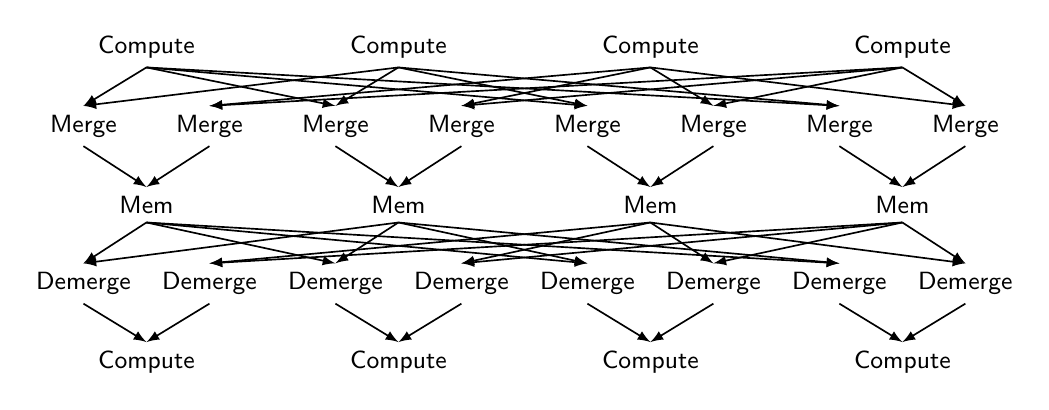
\begin{tikzpicture}[x=1.6cm]
    \foreach \i in {0,...,3} {
      \node (Comp\i-A)   at (2*\i,0)  {Compute};
      \node (Mem\i) at (2*\i,-2) {Mem};
      \node (Comp\i-B) at (2*\i,-4) {Compute};
      \node (DM\i-A0) at (2*\i-0.5,-3) {Demerge};
      \node (DM\i-A1) at (2*\i+0.5,-3) {Demerge};
      \node (M\i-A0) at (2*\i-0.5,-1) {Merge};
      \node (M\i-A1) at (2*\i+0.5,-1) {Merge};
      \draw[arrow] (M\i-A0.south) -- (Mem\i.north);
      \draw[arrow] (M\i-A1.south) -- (Mem\i.north);
      \draw[arrow] (DM\i-A0.south) -- (Comp\i-B.north);
      \draw[arrow] (DM\i-A1.south) -- (Comp\i-B.north);
    }
    \foreach \i in {0,...,3} {
      \draw[arrow] (Comp0-A.south) -- (M\i-A0.north);
      \draw[arrow] (Comp1-A.south) -- (M\i-A0.north);
      \draw[arrow] (Comp2-A.south) -- (M\i-A1.north);
      \draw[arrow] (Comp3-A.south) -- (M\i-A1.north);
      \draw[arrow] (Mem0.south) -- (DM\i-A0.north);
      \draw[arrow] (Mem1.south) -- (DM\i-A0.north);
      \draw[arrow] (Mem2.south) -- (DM\i-A1.north);
      \draw[arrow] (Mem3.south) -- (DM\i-A1.north);
    }
  \end{tikzpicture}
}
\end{frame}
\begin{frame}
  \frametitle{How to merge vectors?}
  \begin{outline}
    \1 Lane-by-lane basis
    \2 Low rate of successful merges
    \pause
    \1 Full crossbar
    \2 Expensive
    \pause
    \1 Restricted crossbar
    \2 Each lane can move one lane to the left or right
    \2 97\% success rate
    \2 Re-use PCU stages for data movement
  \end{outline}
\end{frame}
\begin{frame}
  \frametitle{Preliminary results}
  \begin{outline}
    \1 GEMV-CSR is 2x faster than GPU without optimization
    %pause
    \2 Outer-parallelization will increase speed
    %pause
    \2 GEMV-COO will increase speed
    %\pause
    \2 HBM will increase speed
    \1 Reorder pipeline is roughly 14\% of 6-stage PCU area
    \1 Splitter and merger are <1\% of PCU area
  \end{outline}
\end{frame}
\begin{frame}
  \frametitle{Any questions?}
\end{frame}
\end{document}

\begin{frame}
  \frametitle{PMU issue count (not normalized, to show total cycles)}
  \hskip1.5in\input{../pgf/iter_of.tex}
\end{frame}
\begin{frame}
  \frametitle{Impact of allocator direction (\texttt{if} or \texttt{of})}
  \hskip1.5in\mbox{\pgfplotstableread[col sep=comma]{../../merged_data/iss_hist.csv}\isshist
%\pgfplotstableread[col sep=comma]{merged_data/counters.csv}\counters
\begin{tikzpicture}
\begin{axis}[histstyle]
  \foreach \iter in {1,2} {
    \foreach \ifof in {{if},{of}} {
      \addplot+ [smooth] table [y expr=\thisrow{\iter_\ifof_16_rand_4096_1_0_65536}, x expr=\thisrow{Counts}] {\isshist};
      \addlegendentryexpanded{\iter{} Iter, \ifof}
    }
  }
  \addplot+ [smooth] table [y expr=\thisrow{0_none_16_NA_4096_1_0_65536}, x expr=\thisrow{Counts}] {\isshist};
  :q
  \addlegendentryexpanded{No Stalls}
\end{axis}
\end{tikzpicture}
}
\end{frame}
\begin{frame}
  \frametitle{Impact of allocator randomness}
  \hskip1.5in\pgfplotstableread[col sep=comma]{../../merged_data/iss_hist.csv}\isshist%
\begin{tikzpicture}
\begin{axis}[histstyle]
  \foreach \iter in {1,2} {
    \foreach \ifof in {{if}} {
      \foreach \rand in {{rand},{static}} {
        \addplot+ [smooth] table [y expr=\thisrow{\iter_\ifof_16_\rand_4096_1_0_65536}, x expr=\thisrow{Counts}] {\isshist};
        \addlegendentryexpanded{\iter{} Iter, \ifof, \rand}
      }
    }
  }
  \addplot+ [smooth] table [y expr=\thisrow{0_none_16_NA_4096_1_0_65536}, x expr=\thisrow{Counts}] {\isshist};
  \addlegendentryexpanded{No Stalls}
\end{axis}
\end{tikzpicture}

\end{frame}
\begin{frame}
  \frametitle{Impact of pipeline depth}
  \hskip1.5in
{
\newcommand{\barlen}{5ex}\newcommand{\barmax}{16}{\tiny \settoheight{\zeroheight}{0}\begin{tabu}{rrr@{\hskip.75ex}L{5ex}rr@{\hskip.75ex}L{5ex}rr@{\hskip.75ex}L{5ex}rr@{\hskip.75ex}L{5ex}}
 \toprule
\rowfont{\bfseries\sffamily} & \multicolumn{3}{c}{IF-1-Rand}& \multicolumn{3}{c}{IF-2-Rand}& \multicolumn{3}{c}{No Stalls}& \multicolumn{3}{c}{Augmenting}\\
\cmidrule(l{3pt}r{3pt}){2-4}\cmidrule(l{3pt}r{3pt}){5-7}\cmidrule(l{3pt}r{3pt}){8-10}\cmidrule(l{3pt}r{3pt}){11-13}\rowfont{\bfseries\sffamily} Pipe Depth & Cycles & \multicolumn{2}{c}{Issued}& Cycles & \multicolumn{2}{c}{Issued}& Cycles & \multicolumn{2}{c}{Issued}& Cycles & \multicolumn{2}{c}{Issued}\\ \midrule
1 & \num{513957} & 3.89 & \sparkbar{3.891429}{\barlen}{\barmax}& \num{513971} & 3.89 & \sparkbar{3.891323}{\barlen}{\barmax}& \num{254445} & 7.86 & \sparkbar{7.860371}{\barlen}{\barmax}& \num{513957} & 3.89 & \sparkbar{3.891429}{\barlen}{\barmax}\\
2 & \num{341779} & 5.85 & \sparkbar{5.851954}{\barlen}{\barmax}& \num{328335} & 6.09 & \sparkbar{6.091504}{\barlen}{\barmax}& \num{133299} & 15.00 & \sparkbar{15.004464}{\barlen}{\barmax}& \num{323829} & 6.18 & \sparkbar{6.176331}{\barlen}{\barmax}\\
4 & \num{276567} & 7.23 & \sparkbar{7.232016}{\barlen}{\barmax}& \num{250749} & 7.98 & \sparkbar{7.976574}{\barlen}{\barmax}& \num{133299} & 15.00 & \sparkbar{15.004464}{\barlen}{\barmax}& \num{243276} & 8.22 & \sparkbar{8.221547}{\barlen}{\barmax}\\
8 & \num{261507} & 7.65 & \sparkbar{7.648541}{\barlen}{\barmax}& \num{226729} & 8.82 & \sparkbar{8.821968}{\barlen}{\barmax}& \num{133299} & 15.00 & \sparkbar{15.004464}{\barlen}{\barmax}& \num{220183} & 9.08 & \sparkbar{9.084239}{\barlen}{\barmax}\\
16 & \num{260178} & 7.69 & \sparkbar{7.688375}{\barlen}{\barmax}& \num{216613} & 9.23 & \sparkbar{9.234584}{\barlen}{\barmax}& \num{133299} & 15.00 & \sparkbar{15.004464}{\barlen}{\barmax}& \num{210188} & 9.52 & \sparkbar{9.516828}{\barlen}{\barmax}\\
\midrule 64 & \num{261234} & 7.66 & \sparkbar{7.658448}{\barlen}{\barmax}& \num{215192} & 9.30 & \sparkbar{9.295192}{\barlen}{\barmax}& \num{133299} & 15.00 & \sparkbar{15.004464}{\barlen}{\barmax}& \num{209396} & 9.55 & \sparkbar{9.553778}{\barlen}{\barmax}\\
\bottomrule
\end{tabu}
}
}

\end{frame}
\begin{frame}
  \frametitle{PMU vs. Lock issue rates}
  \hskip1.5in\pgfplotstableread[col sep=comma]{../../merged_data/iss_PMU.csv}\issPMU%
\pgfplotstableread[col sep=comma]{../../merged_data/iss_lock.csv}\isslock%
\begin{tikzpicture}
\begin{axis}[histstyle]
  \foreach \pipedepth in {8, 16, 64} {
    \addplot+ [smooth] table [y expr=\thisrow{\pipedepth-stage}, x expr=\thisrow{iss_PMU}] {\issPMU};
    \addlegendentryexpanded{\pipedepth{} Stages, PMU}
    \addplot+ [smooth] table [y expr=\thisrow{\pipedepth-stage}, x expr=\thisrow{iss_lock}] {\isslock};
    \addlegendentryexpanded{\pipedepth{} Stages, Lock}
  }
  %\addplot+ [smooth] table [y expr=\thisrow{0_none_16_NA}, x expr=\thisrow{Counts}] {\isshist};
  %\addlegendentryexpanded{No Stalls}
\end{axis}
\end{tikzpicture}

\end{frame}
\begin{frame}
  \frametitle{Lock issue rates as a function of subbank count.}
  \hskip1.5in\pgfplotstableread[col sep=comma]{../../merged_data/iss_lock_reqs.csv}\isslock%
\begin{tikzpicture}
\begin{axis}[histstyle]
  %\foreach \subbanks in {4, 16, 64, 256, 1024} {
  \foreach \subbanks in {4, 64, 1024} {
    \addplot+ [smooth] table [y expr=\thisrow{\subbanks-subbanks}, x expr=\thisrow{iss_lock}] {\isslock};
    \addlegendentryexpanded{\subbanks{} sub-banks}
  }
  %\addplot+ [smooth] table [y expr=\thisrow{0_none_16_NA}, x expr=\thisrow{Counts}] {\isshist};
  %\addlegendentryexpanded{No Stalls}
\end{axis}
\end{tikzpicture}

\end{frame}
\begin{frame}
  \frametitle{Impact of allocator type}
  \hskip1.5in\pgfplotstableread[col sep=comma]{../../merged_data/iss_hist.csv}\isshist%
\begin{tikzpicture}
\begin{axis}[histstyle]
  \addplot+ [smooth] table [y expr=\thisrow{3_if_16_rand_4096_1_0_65536}, x expr=\thisrow{Counts}] {\isshist};
  \addlegendentryexpanded{IF-3-R}
  \addplot+ [smooth] table [y expr=\thisrow{1_augmenting_16_rand_4096_1_0_65536}, x expr=\thisrow{Counts}] {\isshist};
  \addlegendentryexpanded{Augmenting}
  \addplot+ [smooth] table [y expr=\thisrow{0_none_16_NA_4096_1_0_65536}, x expr=\thisrow{Counts}] {\isshist};
  \addlegendentryexpanded{No Stalls}
\end{axis}
\end{tikzpicture}

\end{frame}
\begin{frame}
  \frametitle{PMU read and write pipeline occupancy.}
  \hskip1.5in\pgfplotstableread[col sep=comma]{../../merged_data/stage_occ_PMU_pipedepth_read.csv}\occread%
\pgfplotstableread[col sep=comma]{../../merged_data/stage_occ_PMU_pipedepth_write.csv}\occwrite%
\begin{tikzpicture}
  \begin{axis}[histstyle,xlabel={Occupancy},ymax=125000]
  \foreach \pipedepth in {4, 8, 16} {
    \addplot+ [smooth] table [y expr=\thisrow{\pipedepth-pipedepth}, x expr=\thisrow{stage_occ_PMU_2d}] {\occread};
    \addlegendentryexpanded{\pipedepth{} Stages, Read}
    \addplot+ [smooth] table [y expr=\thisrow{\pipedepth-pipedepth}, x expr=\thisrow{stage_occ_PMU_2d}] {\occwrite};
    \addlegendentryexpanded{\pipedepth{} Stages, Write}
  }
  %\addplot+ [smooth] table [y expr=\thisrow{0_none_16_NA}, x expr=\thisrow{Counts}] {\isshist};
  %\addlegendentryexpanded{No Stalls}
\end{axis}
\end{tikzpicture}

\end{frame}
\begin{frame}
  \frametitle{Average separable allocator performance}
  \centering
  {
\newcommand{\barlen}{5ex}\newcommand{\barmax}{16}{\tiny \settoheight{\zeroheight}{0}\begin{tabu}{rrr@{\hskip.75ex}L{5ex}rr@{\hskip.75ex}L{5ex}rr@{\hskip.75ex}L{5ex}rr@{\hskip.75ex}L{5ex}}
 \toprule
\rowfont{\bfseries\sffamily} & \multicolumn{3}{c}{IF-Rand}& \multicolumn{3}{c}{IF-Static}& \multicolumn{3}{c}{OF-Rand}& \multicolumn{3}{c}{OF-Static}\\
\cmidrule(l{3pt}r{3pt}){2-4}\cmidrule(l{3pt}r{3pt}){5-7}\cmidrule(l{3pt}r{3pt}){8-10}\cmidrule(l{3pt}r{3pt}){11-13}\rowfont{\bfseries\sffamily} Iterations & Cycles & \multicolumn{2}{c}{Issued}& Cycles & \multicolumn{2}{c}{Issued}& Cycles & \multicolumn{2}{c}{Issued}& Cycles & \multicolumn{2}{c}{Issued}\\ \midrule
1 & \num{260178} & 7.68 & \sparkbar{7.680000}{\barlen}{\barmax}& \num{349336} & 5.72 & \sparkbar{5.720000}{\barlen}{\barmax}& \num{268456} & 7.45 & \sparkbar{7.450000}{\barlen}{\barmax}& \num{305947} & 6.53 & \sparkbar{6.530000}{\barlen}{\barmax}\\
2 & \num{216613} & 9.23 & \sparkbar{9.230000}{\barlen}{\barmax}& \num{243918} & 8.20 & \sparkbar{8.200000}{\barlen}{\barmax}& \num{218849} & 9.14 & \sparkbar{9.140000}{\barlen}{\barmax}& \num{240053} & 8.33 & \sparkbar{8.330000}{\barlen}{\barmax}\\
3 & \num{215985} & 9.26 & \sparkbar{9.260000}{\barlen}{\barmax}& \num{234354} & 8.53 & \sparkbar{8.530000}{\barlen}{\barmax}& \num{215111} & 9.29 & \sparkbar{9.290000}{\barlen}{\barmax}& \num{235272} & 8.50 & \sparkbar{8.500000}{\barlen}{\barmax}\\
\midrule64 & \num{216077} & 9.25 & \sparkbar{9.250000}{\barlen}{\barmax}& \num{234314} & 8.53 & \sparkbar{8.530000}{\barlen}{\barmax}& \num{214664} & 9.31 & \sparkbar{9.310000}{\barlen}{\barmax}& \num{235284} & 8.50 & \sparkbar{8.500000}{\barlen}{\barmax}\\
\bottomrule
\end{tabu}
}
}

\end{frame}
\begin{frame}
  \frametitle{Impact of pipeline depth}
  \centering
  
{
\newcommand{\barlen}{5ex}\newcommand{\barmax}{16}{\tiny \settoheight{\zeroheight}{0}\begin{tabu}{rrr@{\hskip.75ex}L{5ex}rr@{\hskip.75ex}L{5ex}rr@{\hskip.75ex}L{5ex}rr@{\hskip.75ex}L{5ex}}
 \toprule
\rowfont{\bfseries\sffamily} & \multicolumn{3}{c}{IF-1-Rand}& \multicolumn{3}{c}{IF-2-Rand}& \multicolumn{3}{c}{No Stalls}& \multicolumn{3}{c}{Augmenting}\\
\cmidrule(l{3pt}r{3pt}){2-4}\cmidrule(l{3pt}r{3pt}){5-7}\cmidrule(l{3pt}r{3pt}){8-10}\cmidrule(l{3pt}r{3pt}){11-13}\rowfont{\bfseries\sffamily} Pipe Depth & Cycles & \multicolumn{2}{c}{Issued}& Cycles & \multicolumn{2}{c}{Issued}& Cycles & \multicolumn{2}{c}{Issued}& Cycles & \multicolumn{2}{c}{Issued}\\ \midrule
1 & \num{513957} & 3.89 & \sparkbar{3.891429}{\barlen}{\barmax}& \num{513971} & 3.89 & \sparkbar{3.891323}{\barlen}{\barmax}& \num{254445} & 7.86 & \sparkbar{7.860371}{\barlen}{\barmax}& \num{513957} & 3.89 & \sparkbar{3.891429}{\barlen}{\barmax}\\
2 & \num{341779} & 5.85 & \sparkbar{5.851954}{\barlen}{\barmax}& \num{328335} & 6.09 & \sparkbar{6.091504}{\barlen}{\barmax}& \num{133299} & 15.00 & \sparkbar{15.004464}{\barlen}{\barmax}& \num{323829} & 6.18 & \sparkbar{6.176331}{\barlen}{\barmax}\\
4 & \num{276567} & 7.23 & \sparkbar{7.232016}{\barlen}{\barmax}& \num{250749} & 7.98 & \sparkbar{7.976574}{\barlen}{\barmax}& \num{133299} & 15.00 & \sparkbar{15.004464}{\barlen}{\barmax}& \num{243276} & 8.22 & \sparkbar{8.221547}{\barlen}{\barmax}\\
8 & \num{261507} & 7.65 & \sparkbar{7.648541}{\barlen}{\barmax}& \num{226729} & 8.82 & \sparkbar{8.821968}{\barlen}{\barmax}& \num{133299} & 15.00 & \sparkbar{15.004464}{\barlen}{\barmax}& \num{220183} & 9.08 & \sparkbar{9.084239}{\barlen}{\barmax}\\
16 & \num{260178} & 7.69 & \sparkbar{7.688375}{\barlen}{\barmax}& \num{216613} & 9.23 & \sparkbar{9.234584}{\barlen}{\barmax}& \num{133299} & 15.00 & \sparkbar{15.004464}{\barlen}{\barmax}& \num{210188} & 9.52 & \sparkbar{9.516828}{\barlen}{\barmax}\\
\midrule 64 & \num{261234} & 7.66 & \sparkbar{7.658448}{\barlen}{\barmax}& \num{215192} & 9.30 & \sparkbar{9.295192}{\barlen}{\barmax}& \num{133299} & 15.00 & \sparkbar{15.004464}{\barlen}{\barmax}& \num{209396} & 9.55 & \sparkbar{9.553778}{\barlen}{\barmax}\\
\bottomrule
\end{tabu}
}
}

\end{frame}
%\begin{frame}
  %\frametitle{Impact of access latency (IF-3-Rand)}
  %\centering
  %
{
\newcommand{\barlen}{5ex}\newcommand{\barmax}{16}{\tiny \settoheight{\zeroheight}{0}\begin{tabu}{rrr@{\hskip.75ex}L{5ex}rr@{\hskip.75ex}L{5ex}rr@{\hskip.75ex}L{5ex}rr@{\hskip.75ex}L{5ex}}
 \toprule
\rowfont{\bfseries\sffamily} & \multicolumn{3}{c}{1 Cycles}& \multicolumn{3}{c}{2 Cycles}& \multicolumn{3}{c}{3 Cycles}& \multicolumn{3}{c}{4 Cycles}\\
\cmidrule(l{3pt}r{3pt}){2-4}\cmidrule(l{3pt}r{3pt}){5-7}\cmidrule(l{3pt}r{3pt}){8-10}\cmidrule(l{3pt}r{3pt}){11-13}\rowfont{\bfseries\sffamily} Pipe Depth & Cycles & \multicolumn{2}{c}{Issued}& Cycles & \multicolumn{2}{c}{Issued}& Cycles & \multicolumn{2}{c}{Issued}& Cycles & \multicolumn{2}{c}{Issued}\\ \midrule
1 & \num{513971} & 3.89 & \sparkbar{3.891323}{\barlen}{\barmax}& \num{639837} & 3.13 & \sparkbar{3.125821}{\barlen}{\barmax}& \num{765744} & 2.61 & \sparkbar{2.611860}{\barlen}{\barmax}& \num{891572} & 2.24 & \sparkbar{2.243247}{\barlen}{\barmax}\\
2 & \num{328335} & 6.09 & \sparkbar{6.091504}{\barlen}{\barmax}& \num{385759} & 5.18 & \sparkbar{5.184667}{\barlen}{\barmax}& \num{445195} & 4.49 & \sparkbar{4.492557}{\barlen}{\barmax}& \num{504397} & 3.97 & \sparkbar{3.965194}{\barlen}{\barmax}\\
4 & \num{250749} & 7.98 & \sparkbar{7.976574}{\barlen}{\barmax}& \num{272879} & 7.33 & \sparkbar{7.329479}{\barlen}{\barmax}& \num{297587} & 6.72 & \sparkbar{6.721073}{\barlen}{\barmax}& \num{324495} & 6.16 & \sparkbar{6.163620}{\barlen}{\barmax}\\
8 & \num{226729} & 8.82 & \sparkbar{8.821968}{\barlen}{\barmax}& \num{238853} & 8.37 & \sparkbar{8.374276}{\barlen}{\barmax}& \num{250264} & 7.99 & \sparkbar{7.992276}{\barlen}{\barmax}& \num{262585} & 7.62 & \sparkbar{7.617168}{\barlen}{\barmax}\\
16 & \num{216613} & 9.23 & \sparkbar{9.234584}{\barlen}{\barmax}& \num{224322} & 8.92 & \sparkbar{8.917404}{\barlen}{\barmax}& \num{232586} & 8.60 & \sparkbar{8.600148}{\barlen}{\barmax}& \num{241821} & 8.27 & \sparkbar{8.271742}{\barlen}{\barmax}\\
\midrule 64 & \num{215192} & 9.30 & \sparkbar{9.295192}{\barlen}{\barmax}& \num{221664} & 9.03 & \sparkbar{9.026360}{\barlen}{\barmax}& \num{230224} & 8.69 & \sparkbar{8.689646}{\barlen}{\barmax}& \num{239701} & 8.35 & \sparkbar{8.345706}{\barlen}{\barmax}\\
\bottomrule
\end{tabu}
}
}

%\end{frame}
%\begin{frame}
  %\frametitle{Impact of access latency (Augmenting)}
  %\centering
  %
{
\newcommand{\barlen}{5ex}\newcommand{\barmax}{16}{\tiny \settoheight{\zeroheight}{0}\begin{tabu}{rrr@{\hskip.75ex}L{5ex}rr@{\hskip.75ex}L{5ex}rr@{\hskip.75ex}L{5ex}rr@{\hskip.75ex}L{5ex}}
 \toprule
\rowfont{\bfseries\sffamily} & \multicolumn{3}{c}{1 Cycles}& \multicolumn{3}{c}{2 Cycles}& \multicolumn{3}{c}{3 Cycles}& \multicolumn{3}{c}{4 Cycles}\\
\cmidrule(l{3pt}r{3pt}){2-4}\cmidrule(l{3pt}r{3pt}){5-7}\cmidrule(l{3pt}r{3pt}){8-10}\cmidrule(l{3pt}r{3pt}){11-13}\rowfont{\bfseries\sffamily} Pipe Depth & Cycles & \multicolumn{2}{c}{Issued}& Cycles & \multicolumn{2}{c}{Issued}& Cycles & \multicolumn{2}{c}{Issued}& Cycles & \multicolumn{2}{c}{Issued}\\ \midrule
1 & \num{513957} & 3.89 & \sparkbar{3.891429}{\barlen}{\barmax}& \num{639838} & 3.13 & \sparkbar{3.125816}{\barlen}{\barmax}& \num{765719} & 2.61 & \sparkbar{2.611945}{\barlen}{\barmax}& \num{891600} & 2.24 & \sparkbar{2.243176}{\barlen}{\barmax}\\
2 & \num{323829} & 6.18 & \sparkbar{6.176331}{\barlen}{\barmax}& \num{380775} & 5.25 & \sparkbar{5.252614}{\barlen}{\barmax}& \num{439072} & 4.56 & \sparkbar{4.555207}{\barlen}{\barmax}& \num{498190} & 4.01 & \sparkbar{4.014629}{\barlen}{\barmax}\\
4 & \num{243276} & 8.22 & \sparkbar{8.221547}{\barlen}{\barmax}& \num{265327} & 7.54 & \sparkbar{7.538151}{\barlen}{\barmax}& \num{290058} & 6.90 & \sparkbar{6.895504}{\barlen}{\barmax}& \num{316504} & 6.32 & \sparkbar{6.319339}{\barlen}{\barmax}\\
8 & \num{220183} & 9.08 & \sparkbar{9.084239}{\barlen}{\barmax}& \num{231390} & 8.64 & \sparkbar{8.644310}{\barlen}{\barmax}& \num{242468} & 8.25 & \sparkbar{8.249237}{\barlen}{\barmax}& \num{254671} & 7.85 & \sparkbar{7.853961}{\barlen}{\barmax}\\
16 & \num{210188} & 9.52 & \sparkbar{9.516828}{\barlen}{\barmax}& \num{217953} & 9.18 & \sparkbar{9.177841}{\barlen}{\barmax}& \num{226438} & 8.83 & \sparkbar{8.833637}{\barlen}{\barmax}& \num{235510} & 8.49 & \sparkbar{8.493966}{\barlen}{\barmax}\\
\midrule 64 & \num{209396} & 9.55 & \sparkbar{9.553778}{\barlen}{\barmax}& \num{215383} & 9.29 & \sparkbar{9.288082}{\barlen}{\barmax}& \num{223428} & 8.95 & \sparkbar{8.953779}{\barlen}{\barmax}& \num{232738} & 8.59 & \sparkbar{8.594750}{\barlen}{\barmax}\\
\bottomrule
\end{tabu}
}
}

%\end{frame}
\begin{frame}
  \frametitle{Impact of access latency}
  \centering
  
{
\newcommand{\barlen}{5ex}\newcommand{\barmax}{16}{\tiny \settoheight{\zeroheight}{0}\begin{tabu}{rrrr@{\hskip.75ex}L{5ex}rr@{\hskip.75ex}L{5ex}rr@{\hskip.75ex}L{5ex}rr@{\hskip.75ex}L{5ex}}
 \toprule
\rowfont{\bfseries\sffamily} && \multicolumn{3}{c}{1 Cycles}& \multicolumn{3}{c}{2 Cycles}& \multicolumn{3}{c}{3 Cycles}& \multicolumn{3}{c}{4 Cycles}\\
\cmidrule(l{3pt}r{3pt}){3-5}\cmidrule(l{3pt}r{3pt}){6-8}\cmidrule(l{3pt}r{3pt}){9-11}\cmidrule(l{3pt}r{3pt}){12-14}\rowfont{\bfseries\sffamily} Stages & Alloc. & Cycles & \multicolumn{2}{c}{Issued}& Cycles & \multicolumn{2}{c}{Issued}& Cycles & \multicolumn{2}{c}{Issued}& Cycles & \multicolumn{2}{c}{Issued}\\ \midrule
\multirow{2}{*}{1} & IF & \num{513971} & 3.89 & \sparkbar{3.891323}{\barlen}{\barmax}& \num{639837} & 3.13 & \sparkbar{3.125821}{\barlen}{\barmax}& \num{765744} & 2.61 & \sparkbar{2.611860}{\barlen}{\barmax}& \num{891572} & 2.24 & \sparkbar{2.243247}{\barlen}{\barmax}\\
& Aug & \num{513957} & 3.89 & \sparkbar{3.891429}{\barlen}{\barmax}& \num{639838} & 3.13 & \sparkbar{3.125816}{\barlen}{\barmax}& \num{765719} & 2.61 & \sparkbar{2.611945}{\barlen}{\barmax}& \num{891600} & 2.24 & \sparkbar{2.243176}{\barlen}{\barmax}\\\midrule 
\multirow{2}{*}{2} & IF & \num{328335} & 6.09 & \sparkbar{6.091504}{\barlen}{\barmax}& \num{385759} & 5.18 & \sparkbar{5.184667}{\barlen}{\barmax}& \num{445195} & 4.49 & \sparkbar{4.492557}{\barlen}{\barmax}& \num{504397} & 3.97 & \sparkbar{3.965194}{\barlen}{\barmax}\\
& Aug & \num{323829} & 6.18 & \sparkbar{6.176331}{\barlen}{\barmax}& \num{380775} & 5.25 & \sparkbar{5.252614}{\barlen}{\barmax}& \num{439072} & 4.56 & \sparkbar{4.555207}{\barlen}{\barmax}& \num{498190} & 4.01 & \sparkbar{4.014629}{\barlen}{\barmax}\\\midrule 
\multirow{2}{*}{4} & IF & \num{250749} & 7.98 & \sparkbar{7.976574}{\barlen}{\barmax}& \num{272879} & 7.33 & \sparkbar{7.329479}{\barlen}{\barmax}& \num{297587} & 6.72 & \sparkbar{6.721073}{\barlen}{\barmax}& \num{324495} & 6.16 & \sparkbar{6.163620}{\barlen}{\barmax}\\
& Aug & \num{243276} & 8.22 & \sparkbar{8.221547}{\barlen}{\barmax}& \num{265327} & 7.54 & \sparkbar{7.538151}{\barlen}{\barmax}& \num{290058} & 6.90 & \sparkbar{6.895504}{\barlen}{\barmax}& \num{316504} & 6.32 & \sparkbar{6.319339}{\barlen}{\barmax}\\\midrule 
\multirow{2}{*}{8} & IF & \num{226729} & 8.82 & \sparkbar{8.821968}{\barlen}{\barmax}& \num{238853} & 8.37 & \sparkbar{8.374276}{\barlen}{\barmax}& \num{250264} & 7.99 & \sparkbar{7.992276}{\barlen}{\barmax}& \num{262585} & 7.62 & \sparkbar{7.617168}{\barlen}{\barmax}\\
& Aug & \num{220183} & 9.08 & \sparkbar{9.084239}{\barlen}{\barmax}& \num{231390} & 8.64 & \sparkbar{8.644310}{\barlen}{\barmax}& \num{242468} & 8.25 & \sparkbar{8.249237}{\barlen}{\barmax}& \num{254671} & 7.85 & \sparkbar{7.853961}{\barlen}{\barmax}\\\midrule 
\multirow{2}{*}{16} & IF & \num{216613} & 9.23 & \sparkbar{9.234584}{\barlen}{\barmax}& \num{224322} & 8.92 & \sparkbar{8.917404}{\barlen}{\barmax}& \num{232586} & 8.60 & \sparkbar{8.600148}{\barlen}{\barmax}& \num{241821} & 8.27 & \sparkbar{8.271742}{\barlen}{\barmax}\\
& Aug & \num{210188} & 9.52 & \sparkbar{9.516828}{\barlen}{\barmax}& \num{217953} & 9.18 & \sparkbar{9.177841}{\barlen}{\barmax}& \num{226438} & 8.83 & \sparkbar{8.833637}{\barlen}{\barmax}& \num{235510} & 8.49 & \sparkbar{8.493966}{\barlen}{\barmax}\\\midrule 
\multirow{2}{*}{64} & IF & \num{215192} & 9.30 & \sparkbar{9.295192}{\barlen}{\barmax}& \num{221664} & 9.03 & \sparkbar{9.026360}{\barlen}{\barmax}& \num{230224} & 8.69 & \sparkbar{8.689646}{\barlen}{\barmax}& \num{239701} & 8.35 & \sparkbar{8.345706}{\barlen}{\barmax}\\
& Aug & \num{209396} & 9.55 & \sparkbar{9.553778}{\barlen}{\barmax}& \num{215383} & 9.29 & \sparkbar{9.288082}{\barlen}{\barmax}& \num{223428} & 8.95 & \sparkbar{8.953779}{\barlen}{\barmax}& \num{232738} & 8.59 & \sparkbar{8.594750}{\barlen}{\barmax}\\
\bottomrule
\end{tabu}
}
}

\end{frame}
\begin{frame}
  \frametitle{Impact of lock protector size}
  \centering
  
{
\newcommand{\barlen}{5ex}\newcommand{\barmax}{16}{\tiny \settoheight{\zeroheight}{0}\begin{tabu}{rrrr@{\hskip.75ex}L{5ex}rr@{\hskip.75ex}L{5ex}rr@{\hskip.75ex}L{5ex}rr@{\hskip.75ex}L{5ex}}
 \toprule
\rowfont{\bfseries\sffamily} && \multicolumn{3}{c}{4 Stages}& \multicolumn{3}{c}{8 Stages}& \multicolumn{3}{c}{16 Stages}& \multicolumn{3}{c}{64 Stages}\\
\cmidrule(l{3pt}r{3pt}){3-5}\cmidrule(l{3pt}r{3pt}){6-8}\cmidrule(l{3pt}r{3pt}){9-11}\cmidrule(l{3pt}r{3pt}){12-14}\rowfont{\bfseries\sffamily} Size & Alloc. & Cycles & \multicolumn{2}{c}{Issued}& Cycles & \multicolumn{2}{c}{Issued}& Cycles & \multicolumn{2}{c}{Issued}& Cycles & \multicolumn{2}{c}{Issued}\\ \midrule
\multirow{2}{*}{4} & IF & \num{270601} & 7.39 & \sparkbar{7.391310}{\barlen}{\barmax}& \num{269929} & 7.41 & \sparkbar{7.409793}{\barlen}{\barmax}& \num{270073} & 7.41 & \sparkbar{7.405901}{\barlen}{\barmax}& \num{270073} & 7.41 & \sparkbar{7.405901}{\barlen}{\barmax}\\
& Aug & \num{269390} & 7.42 & \sparkbar{7.424507}{\barlen}{\barmax}& \num{268999} & 7.44 & \sparkbar{7.435266}{\barlen}{\barmax}& \num{269079} & 7.43 & \sparkbar{7.433178}{\barlen}{\barmax}& \num{269079} & 7.43 & \sparkbar{7.433178}{\barlen}{\barmax}\\\midrule 
\multirow{2}{*}{16} & IF & \num{261922} & 7.64 & \sparkbar{7.636186}{\barlen}{\barmax}& \num{259663} & 7.70 & \sparkbar{7.702699}{\barlen}{\barmax}& \num{259497} & 7.71 & \sparkbar{7.707526}{\barlen}{\barmax}& \num{259497} & 7.71 & \sparkbar{7.707526}{\barlen}{\barmax}\\
& Aug & \num{257246} & 7.77 & \sparkbar{7.774997}{\barlen}{\barmax}& \num{255640} & 7.82 & \sparkbar{7.823928}{\barlen}{\barmax}& \num{255635} & 7.82 & \sparkbar{7.824054}{\barlen}{\barmax}& \num{255635} & 7.82 & \sparkbar{7.824054}{\barlen}{\barmax}\\\midrule 
\multirow{2}{*}{64} & IF & \num{253672} & 7.88 & \sparkbar{7.884544}{\barlen}{\barmax}& \num{237179} & 8.43 & \sparkbar{8.432833}{\barlen}{\barmax}& \num{237397} & 8.43 & \sparkbar{8.425161}{\barlen}{\barmax}& \num{237978} & 8.40 & \sparkbar{8.404516}{\barlen}{\barmax}\\
& Aug & \num{246262} & 8.12 & \sparkbar{8.121862}{\barlen}{\barmax}& \num{231453} & 8.64 & \sparkbar{8.641564}{\barlen}{\barmax}& \num{231792} & 8.63 & \sparkbar{8.628956}{\barlen}{\barmax}& \num{231807} & 8.63 & \sparkbar{8.628536}{\barlen}{\barmax}\\\midrule 
\multirow{2}{*}{256} & IF & \num{251256} & 7.96 & \sparkbar{7.960534}{\barlen}{\barmax}& \num{225201} & 8.88 & \sparkbar{8.881697}{\barlen}{\barmax}& \num{219251} & 9.12 & \sparkbar{9.122950}{\barlen}{\barmax}& \num{220259} & 9.08 & \sparkbar{9.082022}{\barlen}{\barmax}\\
& Aug & \num{243808} & 8.20 & \sparkbar{8.203644}{\barlen}{\barmax}& \num{218592} & 9.15 & \sparkbar{9.150188}{\barlen}{\barmax}& \num{212908} & 9.39 & \sparkbar{9.394950}{\barlen}{\barmax}& \num{214634} & 9.32 & \sparkbar{9.320369}{\barlen}{\barmax}\\\midrule 
\multirow{2}{*}{1048576} & IF & \num{250986} & 7.97 & \sparkbar{7.968998}{\barlen}{\barmax}& \num{229478} & 8.72 & \sparkbar{8.716317}{\barlen}{\barmax}& \num{220256} & 9.08 & \sparkbar{9.082254}{\barlen}{\barmax}& \num{215768} & 9.27 & \sparkbar{9.272167}{\barlen}{\barmax}\\
& Aug & \num{243367} & 8.22 & \sparkbar{8.218481}{\barlen}{\barmax}& \num{221450} & 9.03 & \sparkbar{9.032256}{\barlen}{\barmax}& \num{211806} & 9.44 & \sparkbar{9.444166}{\barlen}{\barmax}& \num{208951} & 9.57 & \sparkbar{9.574986}{\barlen}{\barmax}\\
\bottomrule
\end{tabu}
}
}

\end{frame}
\end{document}
